\documentclass[10pt,conference,letterpaper]{IEEEtran}

\usepackage[T1]{fontenc}
\usepackage{cite}
\usepackage{amsmath,amssymb,amsthm}
\usepackage{booktabs}
\usepackage{graphicx}
\usepackage[caption=false,font=footnotesize]{subfig}
\usepackage{multirow}
\usepackage{array}
\usepackage{tabularx}
\usepackage{adjustbox}
\usepackage{float}
\usepackage{url}
\usepackage{xcolor}
\usepackage[unicode,hidelinks]{hyperref}
\usepackage{accsupp}

% Camera-ready revision marks.  Set \showrevfalse before the final upload to
% print the same text in black.
\newif\ifshowrev
\showrevfalse
\newcommand{\rev}[1]{\ifshowrev\textcolor{red}{#1}\else#1\fi}
\newcommand{\revstart}{\ifshowrev\color{red}\fi}

% Keep figure captions visually attached to their figures.  This overrides
% IEEEtran's figure-only caption hook and leaves table-caption spacing intact.
\makeatletter
\renewcommand{\@IEEEfigurecaptionsepspace}{\vskip 2pt\relax}
\makeatother

% Keep the main caption distinct from the final subfigure caption without
% changing the spacing used by single-panel figures.
\newcommand{\subfigmaincaptionskip}{\par\addvspace{4pt}}

\newtheorem{theorem}{Theorem}
\newtheorem{proposition}{Proposition}
\newtheorem{lemma}{Lemma}
\newcommand{\valid}{\textnormal{\textsc{Valid}}}
\newcommand{\explicit}{\textnormal{\textsc{Explicit}}}
\newcommand{\openscope}{\mbox{\textnormal{\textsc{OpenScope}}}}
\newcommand{\invalid}{\textnormal{\textsc{Invalid}}}
\newcommand{\notfound}{\textnormal{\textsc{NotFound}}}
\DeclareRobustCommand{\ssrov}{%
  \texorpdfstring{%
    \mbox{\BeginAccSupp{method=pdfstringdef,unicode,ActualText={S²-ROV}}%
    S\textsuperscript{2}-ROV%
    \EndAccSupp{}}%
  }{S²-ROV}%
}

\hypersetup{pdftitle={Protect the Parent, Spare the Child: Protecting Prefixes in RPKI before All Origins Are Known},pdfauthor={Yuxuan Chen, Chenhui Yu, Hui Zou, Ke Rui, Yanbiao Li, Gaogang Xie}}

\begin{document}

\title{Protect the Parent, Spare the Child: Protecting Prefixes in RPKI before All Origins Are Known}
\author{%
\IEEEauthorblockN{Yuxuan Chen\IEEEauthorrefmark{1}\IEEEauthorrefmark{2},
Chenhui Yu\IEEEauthorrefmark{1}\IEEEauthorrefmark{2},
Hui Zou\IEEEauthorrefmark{1}\IEEEauthorrefmark{2},
Ke Rui\IEEEauthorrefmark{2}\IEEEauthorrefmark{3},
Yanbiao Li\IEEEauthorrefmark{1}\IEEEauthorrefmark{2},
Gaogang Xie\IEEEauthorrefmark{1}\IEEEauthorrefmark{2}}%
\IEEEauthorblockA{\IEEEauthorrefmark{1}Computer Network Information Center, CAS, Beijing, China}%
\IEEEauthorblockA{\IEEEauthorrefmark{2}University of Chinese Academy of Sciences, Beijing, China}%
\IEEEauthorblockA{\IEEEauthorrefmark{3}Institute of Computing Technology, CAS, Beijing, China}%
\IEEEauthorblockA{Email: \{chenyuxuan, chyu, zouhui, lybmath, xie\}@cnic.cn; rui\_ke21b@ict.ac.cn}%
}
\maketitle

\begin{abstract}
Route Origin Validation (ROV) builds on the Resource Public Key Infrastructure (RPKI) through Route Origin Authorizations (ROAs). When the issuer does not yet know which AS will originate a proper subprefix, an aggregate ROA protects the aggregate but makes the resulting unmatched route \invalid{}. A matching ROA still requires the issuer to know and explicitly list that downstream origin in advance. To address this limitation, we introduce Subprefix-Scope ROV (\ssrov{}). It preserves explicit aggregate authorization while adding a holder-signed policy, limited by prefix and maximum route-prefix length, for future proper-subprefix routes without naming downstream origins. We formalize the design, prove strict expressiveness for this dilemma, and evaluate a prototype. With aggregate and downstream ROA issuance each at 50\%, configuring \ssrov{} policies for 80\% of aggregate prefixes leaves 79.1\% fewer conflicting routes on average than conventional ROV. When all 589 ASes in the fixed upgrade set use \ssrov{}, intended-origin delivery reaches 99.2\%, versus 82.1\% under aggregate-only ROV. Operators keep the aggregate ROA and accept an intended subprefix route before a matching ROA lists its origin.
\end{abstract}

\begin{IEEEkeywords}
Routing security, BGP, RPKI, ROV
\end{IEEEkeywords}

\section{Introduction}
\label{sec:introduction}

The Border Gateway Protocol (BGP)~\cite{rfc4271} is the routing foundation of the global Internet, enabling independently operated autonomous systems (ASes) to exchange reachability information for IP prefixes. Yet BGP has no route origin authentication and cannot verify whether an AS is authorized to originate a prefix~\cite{rfc4272,kent2000sbgp}. This gap leaves interdomain routing vulnerable to accidental misoriginations and malicious prefix hijacks that can divert, intercept, or disrupt traffic~\cite{ballani2007hijacking,butler2010bgp}.

To address this gap in origin authorization, the IETF specified the Resource Public Key Infrastructure (RPKI) architecture~\cite{rfc6480} and standardized a profile for Route Origin Authorizations (ROAs)~\cite{rfc9582}. Prefix holders publish ROAs to identify the ASes authorized to originate their prefixes. Routers then use the published ROAs to determine whether the origin of a BGP route is authorized, a process known as Route Origin Validation (ROV)~\cite{rfc6811,rfc8481}. For a route covered by at least one ROA, ROV checks whether a covering ROA authorizes its origin AS and permits its prefix length. If none does, ROV classifies the route as \invalid{}. Depending on local routing policy, an \invalid{} route may be rejected or assigned a lower preference.

An \invalid{} result indicates a conflict with the published ROAs, but not by itself malicious intent~\cite{chung2019,xu2019falsealarm,schulmann2025learning}. A 17-month study classified at least 91\% of daily \invalid{} routes as harmless, and its routing table analysis suggests that rejecting all such routes can eliminate alternative paths and, in some cases, render prefixes unreachable~\cite{righttheship2025}. Transit and IP leasing workflows recur as sources of persistent ROA mismatches, where announcements can precede ROA updates during manual coordination~\cite{demystifying2026}. Intended routing changes can therefore precede a matching ROA: limited visibility of a downstream origin choice creates this gap, and manual reporting extends it. During the gap, ROV labels the intended route \invalid{}, and a policy that filters it can impair reachability.

We focus on a setting in which policy must be installed before the holder knows which origin AS will originate a particular proper subprefix~\cite{demystifying2026,leasing2026}. Figure~\ref{fig:motivation} contrasts the two options available to the holder. Issuing the aggregate ROA, as in Case~1, keeps the aggregate \valid{} but makes a later proper subprefix with a different origin \invalid{}, because no ROA matches that subprefix. Withholding the ROA, as in Case~2, leaves both the aggregate and the subprefix \notfound{}. Conventional ROV therefore cannot keep the aggregate authorized and admit the later route.

\begin{figure}[tb]\centering
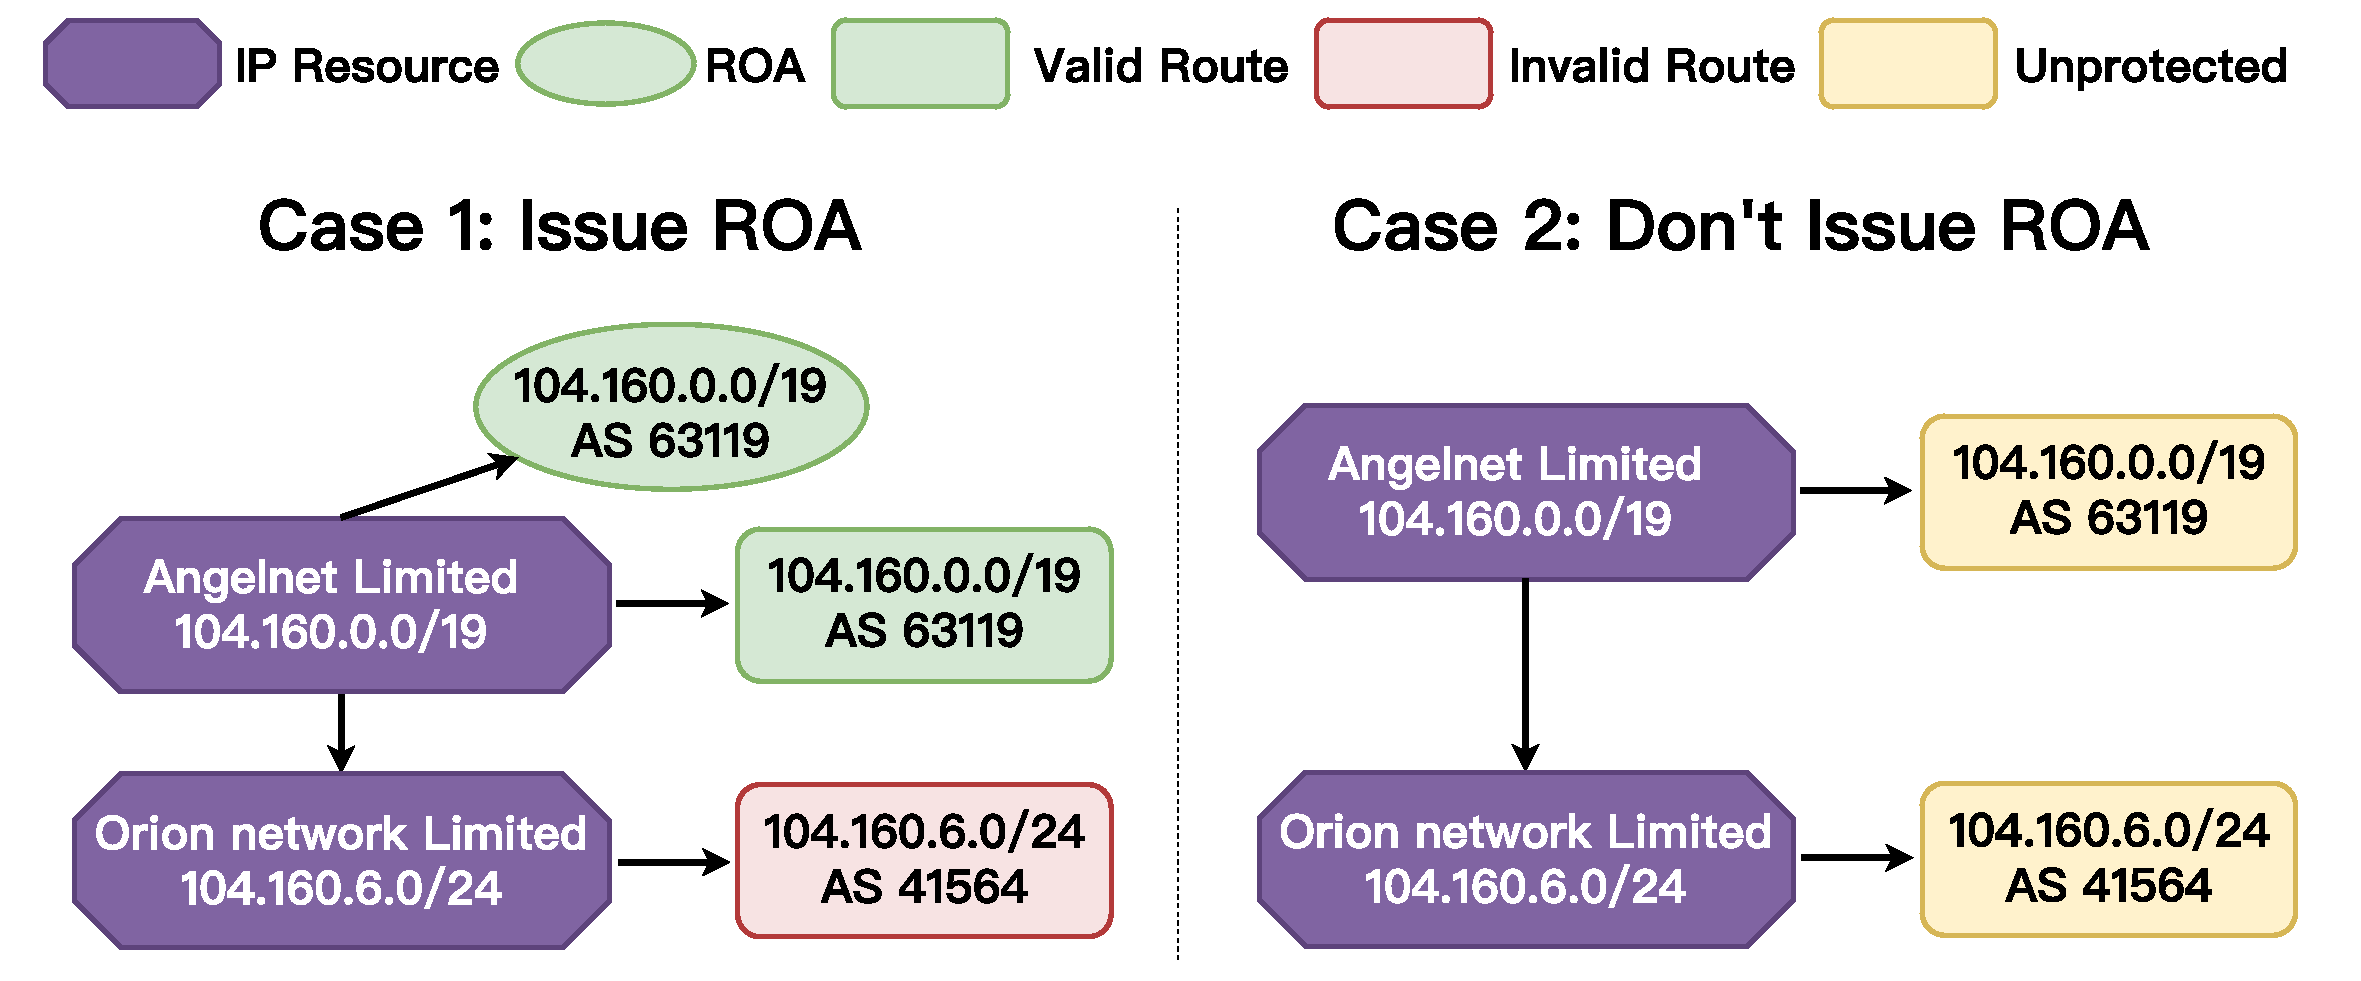
\includegraphics[width=\columnwidth]{figures/fig_motivation}
\caption{Aggregate--subprefix authorization dilemma.}
\label{fig:motivation}\end{figure}

Broadening \emph{maxLength} does not resolve the dilemma because it extends the allowed prefix lengths only for the origin already listed in the ROA~\cite{rfc9319,rfc9582}. An operator can configure local routing policy not to filter the route or use SLURM to override its local RPKI view, but neither approach provides portable policy signed by the holder~\cite{rfc7115,rfc8416}. The wildcard ROA proposal authorizes any AS at its target prefix. Until a regular ROA is issued, a hijacker can therefore announce that prefix and still pass origin validation~\cite{gilad2017rpki}.

In this paper, we introduce Subprefix-Scope ROV (\ssrov{}) to retain explicit origin authorization for an aggregate route with a known origin. It does so without listing every future proper subprefix origin in advance. The holder instead publishes a signed policy that identifies proper-subprefix regions and sets a maximum route-prefix length. If a later route is covered only by this policy, \ssrov{} labels it \openscope{} instead of \invalid{}. Operators can then apply a separate local routing policy to \openscope{} routes, without waiting for reactive publication of an exact ROA.

{\revstart Admitting an intended route in this way also admits an eligible origin that the holder did not select. \ssrov{} records that a route lies below a holder-signed marker and within the policy's length bound; it does not record that the origin is authorized. We therefore present \ssrov{} as a bounded security--availability trade-off rather than as a hijack defense: during the gap, an adversary announcing from an eligible AS inside a marked region receives the same state as the intended origin, and only the local action separates them. Section~\ref{sec:security-scope} states the adversary model, and Section~\ref{sec:eval-security} measures the exposure it creates.}

This paper makes three contributions.
\begin{itemize}
\item We formalize why conventional ROV cannot simultaneously protect an aggregate with a known origin and avoid classifying an unmatched proper subprefix with a different origin as \invalid{} when the downstream origin choice is not yet visible to the issuer.
\item We design \ssrov{}, in which the holder signs prefix markers and a maximum route-prefix length, but no downstream origin list. It preserves conventional ROV semantics and separates the aggregate's \explicit{} state from an eligible descendant's \openscope{} state, making it strictly more expressive for this dilemma.
\item \rev{We ground the problem in observed allocation paths and evaluate an IPv4 and IPv6 prototype across conflicts during partial ROA issuance, system cost, intended-route delivery, unlisted-origin exposure, and the reachability an adversary gains inside a marked region.}
\end{itemize}

To support reproducibility, the implementation, experiment and analysis scripts, configurations, result tables, and figure source data are available at \url{https://github.com/chenyxuan/s2rov-artifact}.

The remainder of the paper is organized as follows. Section~II formalizes the aggregate--subprefix gap and examines downstream-origin visibility and observed allocation paths. \rev{Section~III presents the \ssrov{} design and its security scope, and Section~IV describes the prototype. Section~V reports the evaluation, including the exposure a marked region creates. Sections~VI and~VII discuss related work and the scope of the evidence, respectively, and Section~VIII concludes the paper.}

\section{Aggregate--Subprefix Authorization Gap}
\label{sec:background}

Conventional ROV creates an aggregate--subprefix gap: when an aggregate remains \valid{} and no ROA matches a proper subprefix with a different origin, that route is \invalid{}. We formalize it, examine an operational source and observable pattern, then derive the constraints that guide the design.

\subsection{A Formal Characterization of the Gap}
\label{sec:formal-dilemma}

\emph{ROV model.} A ROA entry is a triple $(q,a,\ell)$ giving prefix $q$, origin $a$, and maximum permitted length $\ell$~\cite{rfc6480,rfc9582}. We write $p\subseteq q$ when $p$ is equal to or more specific than $q$, $p\subset q$ for a proper subprefix, and $|p|$ for the length of $p$. A ROA \emph{covers} route $(p,o)$ when it holds an entry with $p\subseteq q$, and \emph{matches} it when that entry also lists $o=a$ and permits $|p|\leq\ell$. Conventional ROV returns \valid{} if a covering ROA matches, \invalid{} if one covers the route but none matches, and \notfound{} if none covers it~\cite{rfc6811,rfc8481}.

\begin{proposition}[Aggregate--subprefix authorization dilemma]
\label{prop:aggregate-subprefix-dilemma}
Let $(p_0,a_h)$ denote an aggregate route and $(p,o_d)$ a proper subprefix route with a different origin, so $p\subset p_0$ and $o_d\neq a_h$. If conventional ROV classifies $(p_0,a_h)$ as \valid{} under a fixed set of ROAs and no covering ROA in that set matches $(p,o_d)$, then it classifies $(p,o_d)$ as \invalid{}.
\end{proposition}
\begin{proof}
Because $(p_0,a_h)$ is \valid{}, some ROA contains a matching entry $(q,a_h,\ell)$. Thus $p_0\subseteq q$ and $|p_0|\leq\ell$. Since $p\subset p_0\subseteq q$, that ROA also covers $(p,o_d)$, regardless of whether $|p|\leq\ell$; $\ell$ affects matching, not coverage. No covering ROA matches the subprefix route by assumption, so coverage without a match yields \invalid{}.
\end{proof}

\emph{ROV consequence.} Every ROA that matches the aggregate also covers its proper subprefixes, and \emph{maxLength} does not remove that coverage. Preserving $(p_0,a_h)$ as \valid{} while avoiding \invalid{} for $(p,o_d)$ therefore requires a ROA that matches $(p,o_d)$; removing every covering ROA would leave the aggregate \notfound{} (Figure~\ref{fig:motivation}).

\subsection{Observed Aggregate--Subprefix Origin Divergence}
\label{sec:observed-divergence}

Indirect allocation can produce the premise of a missing matching ROA. Suppose $A$ controls ROA issuance for $p_0$, names aggregate origin $a_h$, and allocates space to $B$, which assigns $p\subset p_0$ to $C$ using $o_d\neq a_h$~\cite{rfc6480}. If no channel reports $C$'s choice, $A$ cannot know that $C$ selected $o_d$; IP leasing through a broker exemplifies this pattern~\cite{leasing2026}.

\begin{proposition}[Origin choice visibility limit]
\label{prop:origin-choice-visibility}
Consider two cases that differ only in whether the downstream operator selects $o_1$ or $o_2\neq o_1$ for $p$. If issuer $A$ cannot tell which case occurred, no deterministic ROA policy constructed by $A$ can guarantee both that the selected origin has a matching ROA and that the unselected origin does not.
\end{proposition}
\begin{proof}
Let $L$ be the origins for which $A$ creates matching ROAs for $p$. Because $A$ cannot distinguish the two cases, $L$ is the same in both. If $L$ omits $o_1$ or $o_2$, that origin lacks a matching ROA when selected. If $L$ contains both, it gives the unselected origin a matching ROA in either case.
\end{proof}

Reporting the choice lets $A$ distinguish the cases, and a provisioned downstream issuer can supply the matching ROA directly~\cite{rfc6480,rfc9582}; until either occurs, Proposition~\ref{prop:aggregate-subprefix-dilemma} yields \invalid{} for the later route.

From June 2026 snapshots of the RIPE Database and an RRC00 RIB~\cite{ripe-db,ripe-ris}, we build IPv4 and IPv6 paths along the RIPE status chains, each linking an assigned endpoint prefix to its nearest strictly enclosing allocation prefix, the aggregate prefix, with $d$ counting the intermediate allocations between them. The observations are nested: \emph{RIPE Database} keeps paths with at least one eligible intermediate range, \emph{BGP Data} those with unambiguous origin sets at both ends in RRC00, and \emph{Origin Divergence} those whose origin sets do not overlap.

\begin{table}[t]
\caption{RIPE allocation paths and origin divergence.}
\label{tab:visibility-candidates}
\centering\footnotesize\setlength{\tabcolsep}{3.0pt}

\adjustbox{max width=\columnwidth}{%
\begin{tabular}{@{}llrrrr@{}}\toprule
Version & Observation & $d=1$ & $d=2$ & $d\geq3$ & All \\ \midrule
\multirow{3}{*}{IPv4}
 & RIPE Database & 49,724 & 1,630 & 17 & 51,371 \\
 & BGP Data & 601 & 21 & 0 & 622 \\
 & Origin Divergence & 483 & 21 & 0 & 504 \\ \midrule
\multirow{3}{*}{IPv6}
 & RIPE Database & 48,645 & 65,366 & 8,169 & 122,180 \\
 & BGP Data & 98 & 42 & 0 & 140 \\
 & Origin Divergence & 60 & 23 & 0 & 83 \\ \bottomrule
\end{tabular}}
\end{table}

RIPE records contain paths up to $d=3$ (IPv4) and $d=7$ (IPv6). The RRC00 join observes both endpoints for only 622 of 51,371 IPv4 and 140 of 122,180 IPv6 paths, none at $d\geq3$; within this subset, 504 IPv4 and 83 IPv6 paths show origin divergence, giving 587 candidates under 97 aggregate prefixes.

\subsection{Design Implications}
\label{sec:requirements}

Together, Propositions~\ref{prop:aggregate-subprefix-dilemma} and~\ref{prop:origin-choice-visibility} require a holder-signed policy that keeps the known aggregate origin \explicit{} without listing future proper-subprefix origins: prefix markers plus a maximum route-prefix length, with nonoverlapping markers applying only below that length. Because these fields do not authorize an origin, a qualifying route receives the \openscope{} state, and local policy decides whether to accept, deprefer, or reject it.

\section{\ssrov{} Design}
\label{sec:design}

\ssrov{} uses one holder-signed policy containing a conventional ROA entry and nonoverlapping prefix markers. Each marker applies only to proper subprefixes no longer than the policy's maximum route-prefix length.

\subsection{\ssrov{} Policy}

A policy is
\begin{equation}
D=(v,p_0,m,a_h,\mathcal{R}),
\end{equation}
where $v$ is the profile version, $p_0$ the base prefix, $m$ the maximum route-prefix length, and $a_h$ the known aggregate origin. The policy carries the conventional ROA entry $(p_0,a_h,m)$; $\mathcal{R}$ contains the prefix markers without an origin list.

The current semantics use profile version $v=2$; the address family follows $p_0$, with width $w\in\{32,128\}$ and eligible ASN set $\mathcal{A}$. A valid policy has $|p_0|\leq m\leq w$; every $q\in\mathcal{R}$ is canonical, shares the address family of $p_0$, satisfies $q\subseteq p_0$ and $|q|<m$; and prefixes in $\mathcal{R}$ are disjoint. The tested profile excludes AS~0~\cite{rfc7607}, AS\_TRANS and out-of-range values~\cite{rfc6793}, private~\cite{rfc6996}, documentation~\cite{rfc5398}, and reserved~\cite{iana-as-numbers} values from $\mathcal{A}$; unsupported profiles and mixed address families are invalid.

A marker $q$ covers only proper subprefixes $p\subset q$ with $|p|\leq m$. Marker disjointness makes membership unique; ordinary ROAs may still cover these prefixes.

\subsection{Classification with Provenance}

Let $\rho(p,o)$ be the conventional ROV state of route $(p,o)$ under the validated ROAs, including $(p_0,a_h,m)$. Define the marker-eligibility predicate
\begin{equation}
\mathsf{Scope}_D(p,o)\iff
\begin{aligned}[t]
&|p|\leq m\land o\in\mathcal{A}\setminus\{a_h\}\land{}\\[-2pt]
&\exists q\in\mathcal{R}:p\subset q.
\end{aligned}
\end{equation}
For a valid policy $D$, the complete four-state classifier is
\begingroup
\small
\begin{equation}
\mathsf{State}_D(p,o)=
\begin{cases}
\explicit, & \rho(p,o)=\valid,\\
\openscope, &
\begin{aligned}
&\rho(p,o)=\invalid\\[-2pt]
&{}\land\mathsf{Scope}_D(p,o),
\end{aligned}\\
\invalid, &
\begin{aligned}
&\rho(p,o)=\invalid\\[-2pt]
&{}\land\neg\mathsf{Scope}_D(p,o),
\end{aligned}\\
\notfound, & \rho(p,o)=\notfound.
\end{cases}
\end{equation}
\endgroup
The cases are mutually exclusive and exhaustive, and an exact ROA takes precedence: a matching ROA yields \explicit{}, and an \invalid{} route becomes \openscope{} exactly when $\mathsf{Scope}_D$ holds. The output preserves provenance, because \explicit{} records matching ROA evidence while \openscope{} records marker, length, and ASN eligibility without origin authorization; local policy may accept, deprefer, or reject \openscope{} routes.

\subsection{Properties}

For the aggregate--subprefix dilemma, strict expressiveness requires two properties. With $\mathcal{R}=\varnothing$, \ssrov{} preserves conventional ROV. With markers present, it can return \openscope{} when $\mathsf{Scope}_D$ holds and no ROA matches the downstream origin.

Setting $\mathcal{R}=\varnothing$ gives the preservation condition: the classifier maps conventional \valid{}, \invalid{}, and \notfound{} to \explicit{}, \invalid{}, and \notfound{}, so a conventional entry $(q,a,\ell)$ maps to
\begin{equation}
D=(v,q,\ell,a,\varnothing).
\end{equation}
Discarding $\mathcal{R}$ from any policy leaves its conventional entry $(p_0,a_h,m)$ unchanged, and separately published exact ROAs need no projection to keep providing explicit origin matches.

With $\mathcal{R}$ nonempty, \openscope{} applies only when $p\subset q$ and $|p|\leq m$ for some $q\in\mathcal{R}$ and $o\in\mathcal{A}\setminus\{a_h\}$. Disjointness makes membership unambiguous, and an exact ROA below the same marker still yields \explicit{} because conventional matching comes first.

The following proposition establishes this separation.

\begin{proposition}[Aggregate--subprefix state separation]
\label{prop:scoped-state-separation}
Let
\[
D_{\mathsf{scope}}=(v,p_0,m,a_h,\{p_0\})
\]
be a valid policy. For every proper subprefix $p\subset p_0$ with $|p|\leq m$ and every $o\in\mathcal{A}\setminus\{a_h\}$ for which no ROA matches $(p,o)$,
\[
\begin{aligned}
\mathsf{State}_{D_{\mathsf{scope}}}(p_0,a_h)&=\explicit,\\
\mathsf{State}_{D_{\mathsf{scope}}}(p,o)&=\openscope.
\end{aligned}
\]
The construction is independent of which eligible downstream origin is selected, and the policy does not list that origin.
\end{proposition}

\begin{proof}
The conventional entry $(p_0,a_h,m)$ matches the aggregate route, so its state is \explicit{}. For $(p,o)$, the same entry provides coverage, while the premise excludes a matching ROA. Proposition~\ref{prop:aggregate-subprefix-dilemma} therefore gives the conventional state \invalid{}. Because $p\subset p_0$, $|p|\leq m$, and $o$ is eligible, the marker at $p_0$ satisfies $\mathsf{Scope}_{D_{\mathsf{scope}}}(p,o)$ and the classifier returns \openscope{}.
\end{proof}

The empty marker mapping and Proposition~\ref{prop:scoped-state-separation} satisfy both conditions. Conventional ROV has no state corresponding to \openscope{}, and Proposition~\ref{prop:aggregate-subprefix-dilemma} makes an unmatched proper subprefix with a different origin \invalid{}. Guaranteeing \valid{} for whichever of two indistinguishable origins is selected requires matching both, which Proposition~\ref{prop:origin-choice-visibility} shows also matches the unselected origin. \ssrov{} instead records markers and a length bound without enumerating either origin, so it is strictly more expressive for this dilemma in the stated sense.

\subsection{Security Scope and Threat Model}
\label{sec:security-scope}

{\revstart We consider an adversary that announces routes from AS numbers it controls and knows the policy and its markers, but cannot forge the holder's signature, alter validated RPKI data, or modify the policy. Choosing a prefix $p$ below a marker $q\in\mathcal{R}$ and an eligible origin $o\in\mathcal{A}\setminus\{a_h\}$ with no matching ROA yields \openscope{} instead of \invalid{}, and the receiving network applies its local action. Outside the markers, above $m$, or with an ineligible ASN the route remains \invalid{}, so the adversary gains nothing there.}

{\revstart Three properties bound the exposure: the holder chooses the marked region, so $q\subset p_0$ keeps it inside the aggregate and disjoint markers narrow it; the length bound caps any admitted route; and the eligible ASN set excludes AS~0, AS\_TRANS, and private, documentation, and reserved values. The holder removes the exposure by issuing a matching ROA, which takes precedence, and by shrinking or revoking $\mathcal{R}$; the ROA alone leaves other origins eligible below a retained marker.}

{\revstart The maximum route-prefix length is shared with the conventional entry by construction, so \openscope{} never admits a route longer than the length already authorized for $a_h$: the policy relaxes exactly one field, the origin constraint, and leaves the length envelope unchanged. A separate length bound for the marker branch would admit lengths outside that envelope; we do not evaluate that variant and leave it as an open design choice.}

Section~\ref{sec:implementation} implements this classifier in a reference policy engine and connects validated policies to router enforcement.

\section{Prototype Implementation}
\label{sec:implementation}

The prototype implements the policy path in three stages: policy representation, validation and classification, and route enforcement.

\subsection{Policy Representation}
\label{sec:impl-representation}

The reference engine serializes $D$ canonically for IPv4 and IPv6 replay. Address format tags distinguish the original 14-byte IPv4 header from the IPv6 header, which adds a full 16-byte base address, and remain separate from the profile version bound by the envelope and snapshot. A single flag marks a prefix as a marker: marked records populate $\mathcal{R}$, and unmarked records carry ordinary origin information. Canonical prefixes and sorted origin sets make the encoding independent of input order. Before activation, the parser rejects unsupported versions, mixed address families, noncanonical prefixes, overlapping markers, duplicate keys, invalid ASNs, inconsistent lengths, and trailing bytes. A legacy projection removes the markers and emits the ordinary entries unchanged, so routes matched by those entries remain \explicit{}.

\subsection{Validation and Classification}
\label{sec:impl-engine}

The signed path uses Krill~0.14.4~\cite{krill}, RRDP~\cite{rfc8182}, and Routinator~0.13.2~\cite{routinator}. Experimental Krill adds an \texttt{inclusive} prefix attribute to a fixture derived from a ROA and protected by CMS. Modified Routinator verifies the certification chain and CRL~\cite{rfc6487}, manifest~\cite{rfc9286}, and signed object~\cite{rfc6488}, then exposes validated ordinary and experimental entries through its local JSON API. The engine receives one validated policy with the ordinary entries of the same view, checks covering ordinary entries for an origin and length match, and tests only an otherwise \invalid{} route against the unique applicable marker. One ancestor walk answers that second step, bounded at 33 probes for IPv4 and 129 for IPv6, and the engine returns the state, supporting evidence, and profile version.

\subsection{Route Enforcement}
\label{sec:impl-enforcement}

A Routinator build compatible with legacy clients omits experimental entries from its RFC~8210 RTR output~\cite{rfc8210}, so FRR~10.6.1~\cite{frr} receives only ordinary entries. The compiler reads each neighbor's Adj-RIB-In, extracts the terminal origin, evaluates each prefix, origin, and peer tuple against the selected policy, and rebuilds one inbound route map per neighbor. Clauses match prefix and origin, and a final clause denies the remainder. Recompilation removes stale maps and match objects before attaching the replacement. The action map assigns \explicit{} LP~300, \openscope{} LP~200, \invalid{} rejection, and \notfound{} LP~100 with audit communities. After installation through \texttt{vtysh}, a soft inbound reevaluation applies the replacement to received routes, and the harness checks route presence, rejection, and local preference in the resulting Loc-RIB.

\section{Evaluation}
\label{sec:experiments}

We evaluate \ssrov{} through conflicts on observed allocation paths, system cost and a live path control, routing benefit and exposure, and the reachability an adversary gains.

\subsection{Conflicts during Partial ROA Issuance}
\label{sec:eval-conflict-reduction}

\emph{How does \ssrov{} reduce conflicts during partial ROA issuance?} From Table~\ref{tab:visibility-candidates}, 587 endpoint prefixes yield 589 route--origin pairs under 97 aggregate prefixes, because two IPv4 endpoints have two observed origins; matching ROAs are issued atomically per endpoint and cover its complete observed origin set.

Figure~\ref{fig:partial-policy-coverage} reports the mean share of these pairs classified \invalid{} over 1,000 seeded replays, stepping ROA issuance from 0\% to 100\% in 10\% increments and policy coverage from 0\% to 100\% in 20\% increments under randomized, nested selections. \subref{fig:partial-policy-potential} keeps every aggregate ROA active, while \subref{fig:partial-policy-observed} activates sampled aggregate and downstream ROAs jointly, so an observed conflict needs an active aggregate ROA, an absent downstream ROA, and a route that no applicable policy admits.

\begin{figure}[tb]\centering
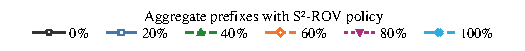
\includegraphics[width=0.9\columnwidth,trim=0 5bp 0 0,clip]{figures/fig_partial_policy_legend}\par
{\captionsetup[subfloat]{farskip=0pt}%
\subfloat[Potential conflicts.]{%
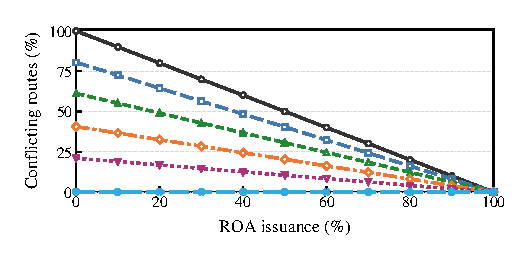
\includegraphics[width=0.9\columnwidth,trim=0 10bp 0 0,clip]{figures/fig_partial_policy_potential}%
\label{fig:partial-policy-potential}}}\par
\subfloat[Observed conflicts.]{%
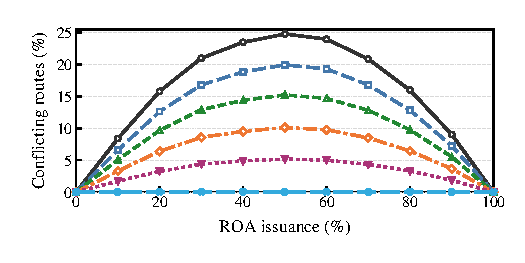
\includegraphics[width=0.9\columnwidth,trim=0 10bp 0 0,clip]{figures/fig_partial_policy_observed}%
\label{fig:partial-policy-observed}}
\subfigmaincaptionskip
\caption{Conflicts during partial ROA issuance.}
\label{fig:partial-policy-coverage}
\end{figure}

At 50\% issuance, conventional ROV leaves mean potential and observed conflict rates of 50.1\% and 24.8\%. Policies on 80\% of the aggregate prefixes lower them to 10.5\% and 5.2\%, relative reductions of 79.1\% in both views; covering all aggregate prefixes leaves 0.1\% and $<0.1\%$ because one observed origin is ineligible, while full downstream issuance makes every route \explicit{}. \ssrov{} therefore lowers both the potential conflicts that aggregate ROAs create and the peak during partial issuance.

\emph{Which aggregate prefixes should be configured for \ssrov{} first?} We keep every aggregate ROA active, fix downstream ROA issuance at 50\% with 293 endpoint bundles per replay, vary the policy share from 0\% to 100\% in 10\% steps, and compare four orders over the same 1,000 selections. Route count orders aggregate prefixes by the eligible observed route--origin pairs they cover; ASRank and AS degree use the customer-cone order and total degree of the observed aggregate origin in the July 2026 CAIDA graph~\cite{luckie2013asrel}, with fixed-seed random tie-breaking; Random reproduces the 50\% slice of Fig.~\ref{fig:partial-policy-coverage}\subref{fig:partial-policy-potential}. Figure~\ref{fig:openscope-placement} reports the four orders as the policy share rises.

\begin{figure}[tb]\centering
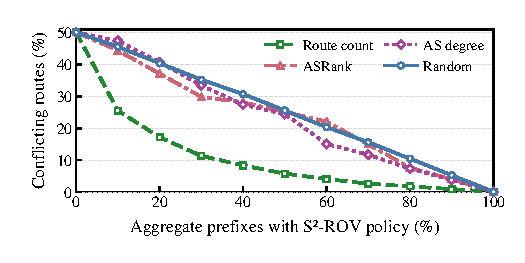
\includegraphics[width=\columnwidth,trim=0 10bp 0 0,clip]{figures/fig_openscope_placement}
\caption{Prioritizing aggregate prefixes for \ssrov{}.}
\label{fig:openscope-placement}
\end{figure}

When 20\% of aggregate prefixes have an \ssrov{} policy, the mean conflict rate is 17.2\% under Route count, against 37.1\% under ASRank, 40.7\% under AS degree, and 40.4\% under Random; at 50\% the rates are 5.8\%, 25.1\%, 24.4\%, and 25.6\%. Prioritizing by eligible observed routes therefore reduces conflicts faster than either AS-topology order on this route set.

\subsection{System Cost and Live Path Control}
\label{sec:eval-cost}

\emph{How do classification and policy update costs scale, and does an installed action persist through a relying party outage?} We replay controlled IPv4 and IPv6 policies and query sets through the reference engine of Section~\ref{sec:impl-engine}, using route and origin pairs from the 24 June 2026 RRC00 RIB~\cite{ripe-ris}. Each policy holds one marked base entry and zero or more noncovering ordinary entries at total sizes of 1, 64, 256, 1,024, and 4,096 records; the single-record condition holds only the marked base entry. Within each IP version the five conditions reuse the same 4,096 queries, which fall below the base marker and return \openscope{}.

Classification times the public classifier with state capture, including CIDR parsing, over 32 warm repeats in five fresh processes pinned to one Kunpeng 920 core under Python~3.12.3.

An update adds the marker to the base entry of an otherwise identical active policy: for each version and size the two immutable snapshots differ only in that marker bit, and timing covers deserialization with validation, canonicalization, and index construction, active replacement, and the fixed route's first \openscope{} classification over 20 fresh processes per cell.

\begin{figure}[tb]\centering
\subfloat[Classification throughput.]{%
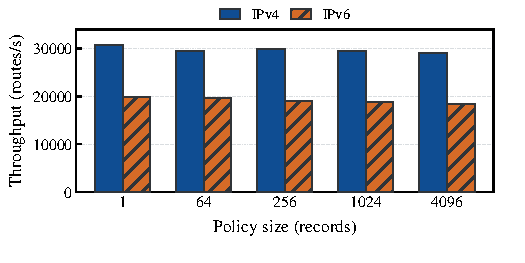
\includegraphics[width=0.85\columnwidth,trim=0 10bp 0 0,clip]{figures/fig_processing_cost_classify}%
\label{fig:processing-cost-classify}}\par
\subfloat[Update latency.]{%
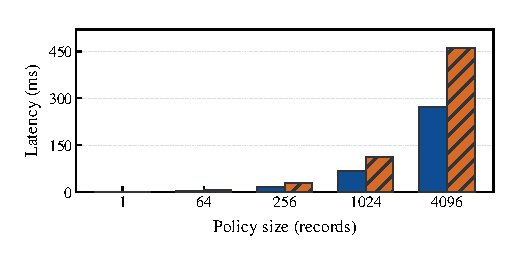
\includegraphics[width=0.85\columnwidth,trim=0 10bp 0 0,clip]{figures/fig_processing_cost_update}%
\label{fig:processing-cost-update}}
\subfigmaincaptionskip
\caption{System cost.}
\label{fig:system-cost}
\end{figure}

Classification throughput ranges from 29,149.8 to 30,647.4 routes/s for IPv4 and from 18,346.0 to 19,794.3 routes/s for IPv6 across the five sizes.

Figure~\ref{fig:system-cost}\subref{fig:processing-cost-update} reports update latency: it rises from 0.3 to 273.0\,ms for IPv4 and from 0.5 to 459.0\,ms for IPv6 across the same sizes, staying below 0.5\,s at 4,096 records. In the live path control, we interrupt the relying party for 15\,s after action installation, and the last installed action remains effective throughout the outage.

\subsection{Reachability and Origin Exposure}
\label{sec:eval-consequences}

\emph{How do intended route reachability and eligible unlisted origin exposure vary as more ASes are upgraded?} Deployment is the share of a fixed 589-AS upgrade set using \ssrov{} within a retained 77,429-AS BGPy graph~\cite{bgpy2023,gaorexford2001}. We evaluate 200 sampled aggregate-prefix cases in 10\% increments under five fixed upgrade orders; each pairs an aggregate with a proper subprefix originated by another AS. Section~\ref{sec:eval-conflict-reduction} instead varies ROA issuance and aggregate-prefix policy coverage.

The panels use different announcement sets and compare \ssrov{} with two conventional baselines: aggregate-only ROV, which uses only the aggregate ROA, and exact-match ROV, which lists the intended subprefix and its origin AS. Delivery is the percentage of the 77,429 topology ASes whose selected path ends at the plotted origin. \subref{fig:deployment-intended} reports intended-origin delivery; \subref{fig:deployment-competition} adds one eligible unlisted origin sampled uniformly per case and reports its delivery. \ssrov{} results average five fixed upgrade orders, and we report absolute percentages.

\begin{figure}[tb]\centering
\subfloat[Intended route delivery.]{%
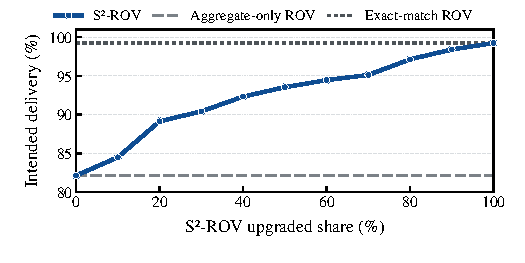
\includegraphics[width=0.95\columnwidth,trim=0 10bp 0 0,clip]{figures/fig_deployment_outcomes_a}%
\label{fig:deployment-intended}}\par
\subfloat[Unlisted origin delivery.]{%
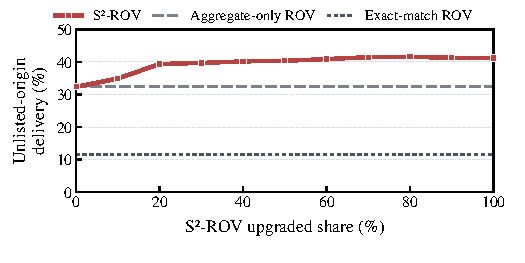
\includegraphics[width=0.95\columnwidth,trim=0 10bp 0 0,clip]{figures/fig_deployment_outcomes_b}%
\label{fig:deployment-competition}}
\subfigmaincaptionskip
\caption{Reachability and origin exposure.}
\label{fig:deployment-outcomes}
\end{figure}

At 50\% of the fixed upgrade set, \ssrov{} raises intended route delivery from 82.1\% under aggregate-only ROV to 93.5\%, while exact-match ROV reaches 99.2\%. In the competition setting it raises unlisted origin delivery from 32.4\% to 40.3\%; exact-match ROV yields 11.7\%.

When all 589 ASes in the set use \ssrov{}, intended route delivery reaches 99.2\%, matching exact-match ROV, while aggregate-only ROV remains at 82.1\%. Unlisted origin delivery rises from 32.4\% to 41.2\%, whereas exact-match ROV lowers it from 32.4\% to 11.7\%. The \ssrov{} value reaches 41.6\% at 80\% and declines to 41.2\% at 100\%.

A separate IPv6 candidate sensitivity evaluates the 0\%, 50\%, and 100\% endpoints for 21 distinct origin pairs from Table~\ref{tab:visibility-candidates}, yielding 210 scenarios across eight aggregate prefixes; at 100\%, every intended-only case matches the exact-match ROV reference. Relative to aggregate-only ROV, these eight aggregates gain 18.7 on average in intended delivery and 17.6 in unlisted-origin exposure in the separate competition setting, while the median change across pairs is 0.0 and 14.0.

\subsection{Attack Reachability}
\label{sec:eval-security}

{\revstart \emph{What does a marked region admit to an adversary?} We reuse the routing model of Section~\ref{sec:eval-consequences} and add a same-length sibling prefix announced by the adversary: the other child of the leaf's supernet at the leaf's prefix length. Conventional authorization remains one aggregate ROA for the aggregate origin with \texttt{maxLength} equal to the aggregate length; the treatment configures an \ssrov{} policy for all 589 ASes in the upgrade set and maps \openscope{} to acceptance. Each of the 200 sampled units runs in both cells, giving 600 trials under the same stratification and weights.}

{\revstart Within the 589 upgrading ASes, the adversary's sibling route is selected by 0.0\% of them under conventional ROV and by 98.6\% once every AS in the set runs \ssrov{}. Across all 77,429 modeled ASes reachability rises from 51.7\% to 98.2\%; the conventional value is not zero because ASes outside the upgrade set do not filter. Destination-level attribution to the adversary rises from 68.0\% to 98.2\%. This is the measured cost of the state: inside a marked region the upgrade set no longer separates the adversary from the intended origin, and only the local action does.}

{\revstart \emph{How much does the local action matter?} The routing model applies one admission decision per state, so these outcomes correspond to accepting \openscope{}. Rejecting it reproduces the aggregate-only ROV outcomes by construction, since an \openscope{} route is one that no ROA matches: 82.1\% intended delivery and 32.4\% unlisted-origin delivery. The two measured endpoints therefore bracket the action spectrum at the level of admission. A preference between them would matter only where an \openscope{} route competes for the same prefix with an \explicit{} route from a different origin, which neither announcement set here produces; the prototype assigns LP~300 to \explicit{} and LP~200 to \openscope{}, so a matching ROA wins once it exists.}

{\revstart \emph{Scope of these counts.} All 589 pairs in the conflict replay are covered by at least one ROA, so \notfound{} does not enter that estimand; the classifier leaves \notfound{} unchanged, whereas withdrawing the covering entry would move a route to \notfound{} while also withdrawing the aggregate's \explicit{} evidence (Case~2 of Figure~\ref{fig:motivation}). Both reported baselines are therefore ROV configurations rather than a no-RPKI arm.}

\section{Related Work}
\label{sec:related_work}

\subsection{RPKI Measurements and Failure Modes}

Longitudinal studies measure ROA coverage and invalid route origins~\cite{chung2019}, while passive and controlled methods infer whether networks filter invalid announcements~\cite{gilad2017rpki,hlavacek2023}. Later work traces conflicts to misconfiguration, changing origins, leasing, and operational coordination~\cite{demystifying2026,leasing2026}, and broader analyses cover repository, validator, and router security~\cite{sok2025} and the collateral damage of filtering~\cite{improv2025}. Conflicts therefore have heterogeneous causes; we address the preceding policy problem of specifying holder-signed prefix and length limits before a downstream origin is selected or reported.

\subsection{Conflict Diagnosis and Mitigation}

Diagnosis methods treat this heterogeneity as an inference problem. Early work classifies false alarms among routes that RPKI marks invalid~\cite{xu2019falsealarm}. SROV uses route duration and registry, routing, DNS, and data plane evidence to distinguish errors from hijacks~\cite{srov2022}; LOV combines a classifier, AS-visibility analysis, and quarantine into a benign-route whitelist~\cite{schulmann2025learning}; and Right the Ship assesses legitimacy from organization, path, and competition evidence~\cite{righttheship2025}. These systems decide whether a conflict should be tolerated; none changes the signed policy available before a downstream origin is known.

\subsection{Authorization and Validation Mechanisms}

Operational guidance favors narrow ROAs for known origins, while delegated certification lets a provisioned downstream holder publish an exact ROA~\cite{rfc7115,rfc9319,rfc6480,rfc6487,rfc9582}. Wildcard ROA provides policy signed by the holder for any origin at its target prefix, with a regular ROA taking priority~\cite{gilad2017rpki}. SLURM supplies local exceptions~\cite{rfc8416}; Hybrid ROA compresses origin lists~\cite{hybridroa2024}; Signed Prefix Lists enumerate prefixes without conveying holder permission~\cite{rpki-spl2025}; DISCO changes the validation path~\cite{disco2020}; and BGPsec and ASPA add path or provider evidence~\cite{rfc8205,aspa-profile2026}. None encodes a holder-signed proper-subprefix region with a maximum length as a separate validation input.

\section{Discussion}
\label{sec:discussion}

{\revstart \emph{Security.} Inside a marked region, an intended origin and an eligible unlisted origin receive the same \openscope{} state. That state records two facts: the route falls below a holder-signed marker, and its length stays within the policy bound. It does not record that the origin is authorized, and an exact ROA still takes precedence. Section~\ref{sec:security-scope} states the adversary model, and Section~\ref{sec:eval-security} measures the reachability the state creates. The operator-facing decision is therefore narrow: which regions to mark, and which local action to apply. Because the state is reported explicitly, a router can count or log \openscope{} admissions separately from authorized routes and revisit the region once the traffic pattern settles.}

{\revstart \emph{What the conflict rates express.} At 80\% policy coverage, the relative reduction approaches the coverage itself, because a marked aggregate contributes no descendant conflict unless its origin is ineligible. The 79.1\% figure is therefore an internal-consistency check that states the size of the uncovered remainder, 10.5\% and 5.2\%, rather than an independently estimated effect. The replay uses 589 route--origin pairs under 97 aggregate prefixes from a single RRC00 snapshot. It characterizes that observed set, and it does not estimate Internet-wide rates. Reporting the absolute residual rates alongside the relative change keeps that distinction visible.}

{\revstart \emph{What the routing model supports.} The model fixes one 77,429-AS graph, one 589-AS upgrade set, 200 sampled units, and five upgrade orders. The intended-only and competition panels isolate benefit from exposure, but they remain separate conditional comparisons rather than a same-scenario frontier. The IPv6 sensitivity likewise leaves the median intended-delivery change at 0.0. Traffic, operator intent, another topology, and another ROV set all remain outside the evidence. The two panels answer separate questions: whether the intended route is reachable, and what else becomes reachable beside it.}

{\revstart \emph{Deployment path.} Holders place nonoverlapping markers before a matching ROA exists, operators map \openscope{} to a chosen local action, and exact ROAs authorize the origin once it is known. On the observed route set, prioritizing aggregates by the eligible route--origin pairs they cover reduces conflicts faster than ASRank, AS degree, or random ordering. A holder narrows a marked region by replacing one broad marker with disjoint markers on the intended subtrees. Once the matching ROA is in force, revoking the marker closes the region without touching the aggregate entry.}

\section{Conclusion}
\label{sec:conclusion}

This paper addresses a gap in ROV: a holder may know the aggregate origin before the origin of an intended proper subprefix. \ssrov{} preserves explicit aggregate authorization through holder-signed prefix markers and a length bound without enumerating downstream origins. Formal analysis shows strict expressiveness for this setting, and the evaluation shows fewer conflicts during partial ROA issuance and greater intended-origin delivery. Because the policy also applies to eligible unlisted origins, operators choose how to treat those routes until a matching ROA is issued.


\section*{Acknowledgment}

This work was supported by the National Natural Science Foundation of China
under Grant No.~62302476.

\bibliographystyle{IEEEtran}
\bibliography{refs}

\end{document}
